\documentclass[fleqn,onecolumn,a4paper,12pt,titlepage]{article}
\usepackage[showcrop]{geometry}
\geometry{textheight=25.0cm,textwidth=17.0cm,headheight=3cm,headsep=0.5em}%hmargin=4.2cm
\usepackage{graphicx}%[dvips,pdftex]
\usepackage{amssymb}
\usepackage{amsmath}%centertags
\usepackage[T1]{fontenc}
\usepackage[polish]{babel}
\usepackage{float}
\usepackage[final]{listingsutf8}
\usepackage{fancyhdr}
\usepackage{tikz}
\usepackage{caption}
\usepackage{hyperref}
\usepackage{datetime2}
\usepackage{enumitem}
\usepackage{blindtext}

\pagestyle{fancy}
\fancyfoot[L,R]{\tiny{\texttt{\symbol{64}}  built: \today{} at \DTMcurrenttime}} 

\begin{document}

\begin{titlepage}
    
\includegraphics[width=0.25\textwidth]{kai.png}\par\vspace{3cm}
    \centering
    {\LARGE \textsc{Narzędzia dla programistów} \par}
    \vspace{2cm}
    {\Large \textsc{Laboratorium 1} \par} % NALEŻY UZUPEŁNIĆ
    \vspace{2cm}
    {\textsc{Wprowadzenie} \par} % NALEŻY UZUPEŁNIĆ
    \vfill
    Mikołaj Hus $-$ 179503 $-$ L00 \par % NALEŻY UZUPEŁNIĆ
    \vspace{2cm}
    {\large {\today} \par}
\end{titlepage}

\section*{Zadanie 1}

Zapoznanie się z interfejsem graficznym MacOS.

\section*{Zadanie 2}

Zapoznanie się z aplikacją \textit{Finder}.

\section*{Zadanie 3}

Przenoszenie i kopiowanie pilków w aplikacji \textit{Finder}.

\section*{Zadanie 5}

Uruchomienie \textit{Launchera} systemu MacOS.

\section*{Zadanie 6}

Uruchomienie aplikacja \textit{TextEdit} i utworzenie przkładowego pliku tekstowego.

\section*{Zadanie 7}

Zlokalizowanie utworzenie pliku za pomocą \textit{Findera}.

\section*{Zadanie 8}

Podgląd pliku tekstowego.

\section*{Zadanie 9}

Kopiowanie pliku tekstowego.

\section*{Zadanie 10}

Otworzenie pliku tekstowego za pomocą aplikacji \textit{Pages} i zmodyfikowanie go.

\section*{Zadanie 12}

Przełączanie się między oknami aplikacji.

\section*{Zadanie 14}

Testowanie skórót klawiszowych podczas edycji tekstu.

\section*{Zadanie 17}

Sprawdzenie struktury programów w systemie MacOS.

\section*{Zadanie 19-23}

Sprawdzenie zainstalowanego oprogramowania.\\
Oprogramowanie zainstalowane poprawnie.

\section*{Zadanie 24}

Uruchomienie aplikacji \textit{Terminal}.

\section*{Zadanie 25-27}

Sprawdzenie wersji \textit{Xcode}, \textit{LATEX} oraz \textit{Git}

\section*{Zadanie 28-32}

Oczyszczenie stanowiska pracy.

\newpage

\section*{Zadanie 34}

Wygenerowanie obrazu prze ChatGPT.
\begin{figure}[H]%
    \centering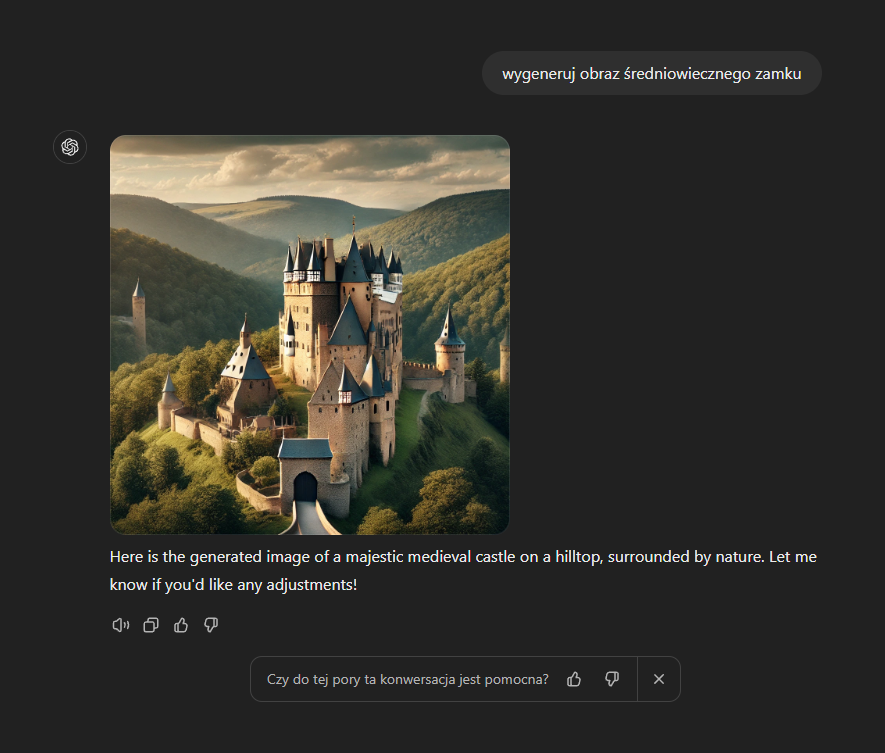
\includegraphics[width=0.9\textwidth]{gen01.png}
    \caption{Wygenerowany obraz}
    \label{fig:obraz wygenerowany przez ChatGPT}
\end{figure}

\newpage

\section*{Zadanie 34}

Implementacja algorytmu plecakowego wykonana prze ChatGPT

\begin{figure}[H]%
    \centering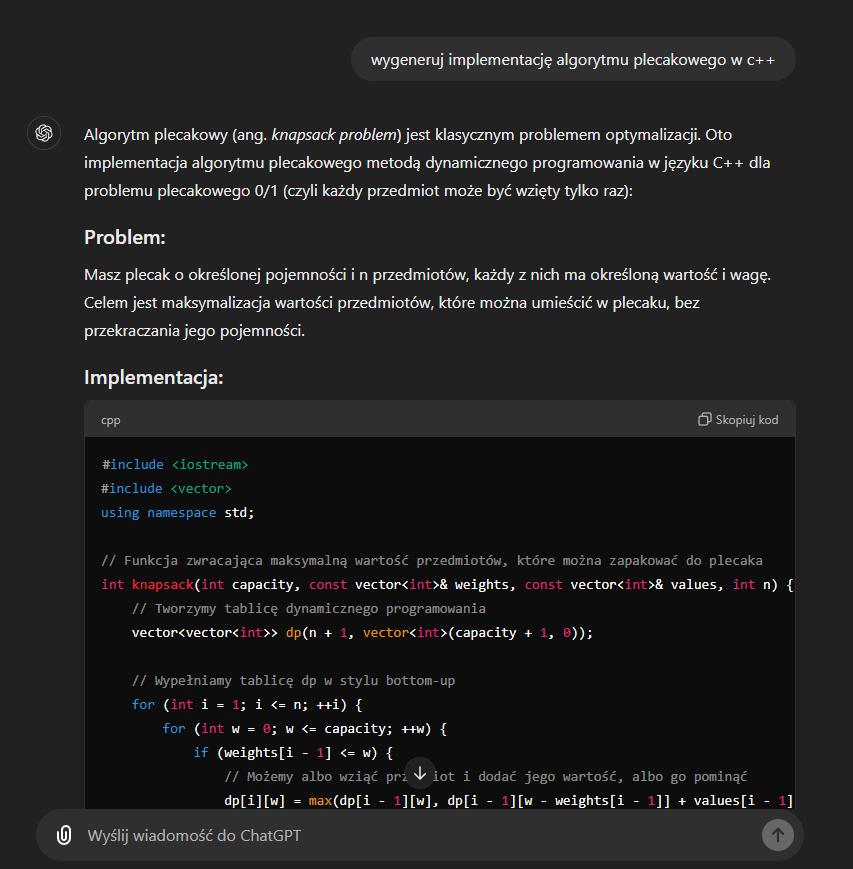
\includegraphics[width=0.9\textwidth]{gen02.png}
    \label{fig:algorytm plecakowy}
\end{figure}
\begin{figure}[H]%
    \centering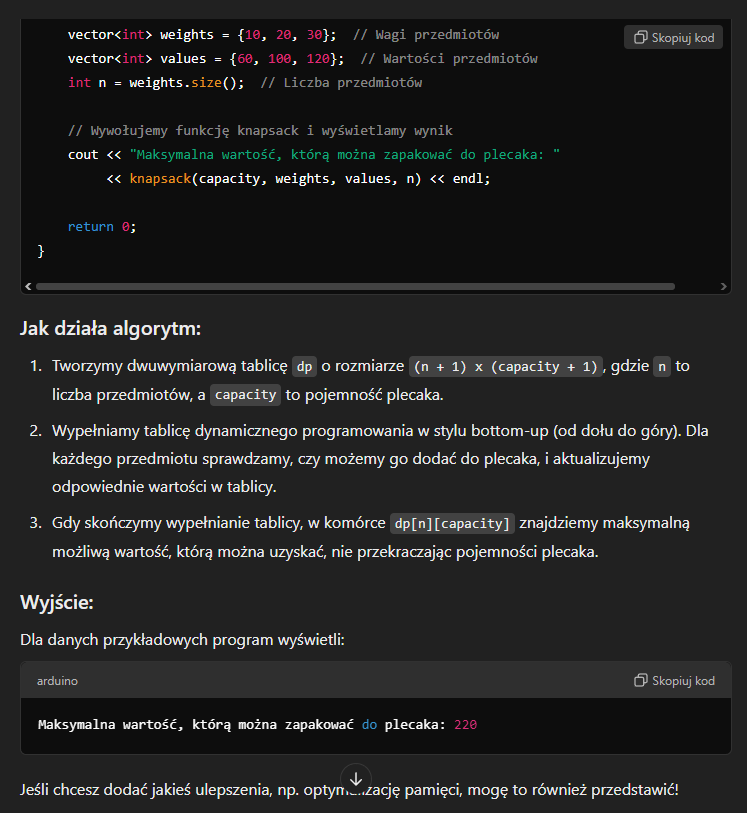
\includegraphics[width=0.9\textwidth]{gen03.png}
    \caption{implementacja algorytmu plecakowego}
    \label{fig:algorytm plecakowy}
\end{figure}

Odpowiedź wygenerowana przez ChatGPT jest w stanie w perwnym stopniu pomóc przy nauce języka C++.

\end{document}